Square signals are multi-frequency signals. Taking their Fourier transform, it is possible to see that a square wave is composed of a fundamental frequency followed by odd-frequency harmonics with decreasing amplitudes \cite{Subhan2019}. An ideal symmetrical square wave of amplitude 2 with peaks at -1 and 1 \cite{ramaley1969theory} follows this equation:
\begin{equation}
   x(t) = \frac{8}{\pi} (sin(\omega t) + \frac{1}{3} sin(3 \omega t) + \frac{1}{5} sin(5 \omega t) + \frac{1}{7} sin(7 \omega t) + \dots)
\end{equation}
Such a geometrical sum can be better shown as follows \cite{Subhan2019,ramaley1969theory}:
\begin{equation}
\label{eq:Squarewave}
   x(t) = \frac{8}{\pi} \displaystyle\sum_{n=1,3,5,7...} ^{\infty} \frac{(sin(n \omega t)}{n} 
\end{equation}
An important point to note from this equation and from \autoref{fig:SquareWave} is that the amplitude of the fundamental differs from the one of a sinewave of amplitude 2 \cite{ramaley1969theory}. Such a difference $\frac{8}{\pi} \neq 2$ will affect the measurements later on, but can be corrected in post-processing (see \autoref{sec:ImpedancePrinciples}) \cite{Subhan2019}. 
\begin{figure}[h]
    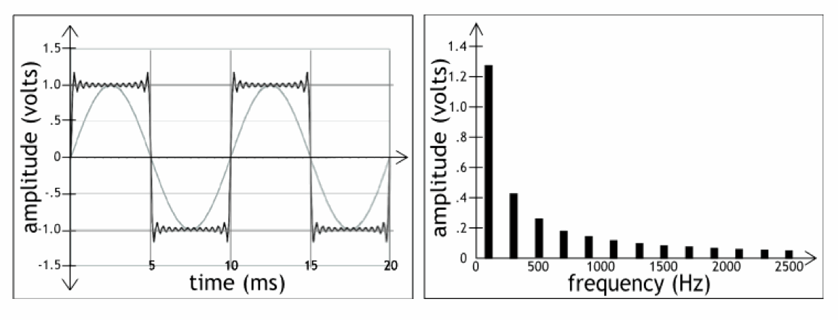
\includegraphics[width=1\textwidth]{SquareWave}
    \caption{Symmetrical practical square-wave of amplitude two described as a function of time and frequency.}
    \label{fig:SquareWave}
\end{figure}